\documentclass[conf]{new-aiaa}

\usepackage{float}
\usepackage{subfigure}
\usepackage[justification=centering]{caption}
\usepackage{multirow} \usepackage{graphicx}
\graphicspath{ {./images/} }
\usepackage{nameref}
\usepackage{amsmath}
\usepackage{amssymb}
\usepackage{amsfonts}
\usepackage[linesnumbered,ruled]{algorithm2e}
\usepackage{tikz}
\usetikzlibrary{calc,patterns,decorations.pathmorphing,decorations.markings,positioning,automata,shapes,arrows}
\tikzstyle{block} = [rectangle, draw, text width=3.5cm]
\tikzstyle{line} = [draw, -latex']
\usepackage{pgfplots}
\usepgfplotslibrary{colormaps,external}
\usepackage{ulem}
\usepackage{verbatim}
\usepackage[version=4]{mhchem}
\usepackage{siunitx}
\usepackage{pbox}
\usepackage{longtable,tabularx}
\setlength\LTleft{0pt} 

\title{Automated Placement of Wing and Fuselage 
      Internal Structures Guided by Finite Element Analysis}

\author{Justin L. Clough%
        \footnote{
          PhD Student, 
          Aerospace and Mechanical Engineering Department, 
          854 Downey Way, RRB 101.}
        and Assad A. Oberai%
        \footnote{  
          Professor, 
          Aerospace and Mechanical Engineering Department, 
          854 Downey Way, RRB 101.}}
\affil{University of Southern California,
       Los Angeles, CA, 90089}
\author{Andrew J. Zakrajsek%
        \footnote{
          Research Engineer,
          Air Force Research Laboratory, AFRL/RQ
          Bldg. 45, 2130 Eighth Street,
          Wright-Patterson AFB, OH 45433.}}
\affil{AFRL/RQHV, Wright-Patterson AFB,
       Dayton, OH, 45433}

\begin{document}
\maketitle

\begin{abstract}
The global layout of the structure is typically not addressed
in the early conceptual phase of aircraft design.
The external geometry is usually finished before the 
internal structure is even initialized.
This leads to errors between the predicted and 
actual performance of the realized vehicle as well as
complications in the later design phases.
This work details and demonstrates extensions
to the \texttt{GRASP} program which automatically 
creates frame layouts for wings and fuselages
with traditional components: ribs, spars, bulkheads, and longerons.
A user needs to design only the outer mold line of the 
vehicle, specify a expected vehicle weight, 
define material properties,
and define an allowable maximum deflection.
A branch-and-cut style algorithm was used
to traverse the integer space of 
different design configurations.
Each design configuration is automatically
created with a parametric geometry kernel,
discretized into a Finite Element (FE) mesh,
and used in a FE analysis to determine 
parameters of interest using all open source software.
This automated work flow is demonstrated with the 
geometry of the X-15 aeroplane.
Variations of this geometry are also evaluated
to show the ability of the work flow to 
handle parametric geometry definitions.
\end{abstract}

\section{Nomenclature}

{\renewcommand\arraystretch{1.0}
\noindent\begin{longtable*}{@{}l @{\quad=\quad} l@{}}
GRASP & Guided Rib And Spar Placement \\
MER   & Mass Estimating Relations \\
FE    & Finite Element \\
% AM    & Additive Manufacturing \\
OML   & Outer Mold Line \\
ESP   & Engineering Sketch Pad
\end{longtable*}}

\section{Introduction}
The conceptual design of modern aerospace systems is grounded in 
various multi-disciplinary design processes. 
These conceptual designs typically focus on the aerodynamic performance, 
weight assumptions, trajectory analysis, and overall ability of the 
system to meet the design requirements. 
A key discipline missing from the majority of early conceptual design, 
is the global structural design. 
This is due to the complex nature and knowledge required to 
design the internal structural layout of a new aerospace system 
\cite{horvath_aircraft_conceptual_structural_design_using_AMMIT,
      alyanak_efficient_supersonic_air_cehicle_structural_modeling,
      sensmeier_automatic_aircraft_structural_topology_generation_for_multidisc}.
Compounding this complexity is the ever changing vehicle 
geometry during the conceptual design phase, 
mainly due to recent advances in parametric geometry. 
Due to the early design fluidity, 
the conceptual structural design has been mainly incorporated in design 
loops through material selection and the resulting empirical 
Mass Estimating Relations (MERs) 
\cite{horvath_aircraft_conceptual_structural_design_using_AMMIT}.
These relations are used until the conceptual design is nearly finalized, 
which then initializes the structural design. 
The structural design typically starts with rough hand calculations, 
up to Finite Element (FE) methods, and eventual structural testing. 
At this point in the design cycle it is typically too late to greatly 
affect the overall system design 
\cite{alyanak_efficient_supersonic_air_cehicle_structural_modeling}.
Therefore, the final conceptual design can complicate the structural 
design and result in increased weight or reduced efficiency of the system. 
The early incorporation of structural design is important for understanding 
the proposed system's feasibility, generating accurate weight predictions, 
assisting the multi-disciplinary design trade space exploration, 
and guiding the system to an optimal solution.

The work presented here has the goal of highlighting the most 
advantageous method to achieve early automated structural conceptual 
designs, within the multi-disciplinary design loop 
independent of direct structural designer expertise. 
To accomplish this the automated layout process needs an OML input, 
design loads, and objective (i.e., minimize wing deflection below an allowable amount). 
The automation framework is then linked to the same parametric geometry 
engine, a layout generation method, FE analysis, and a tailorable framework. 
The resulting work highlights how an 
automated conceptual design framework was setup to automate a 
structure layout for wing and fuselages without any input from the structural designer. 

Note to the reviewers: A more extensive review of the 
state of the art will be included in the 
final manuscript.

\section{Methods} \label{sec_methods}
This project's goal was to extend the features of the original \texttt{GRASP}
program to also layout fuselage frames.
The total frame now includes ribs and spars in the wing, a wing root cap,
and bulkheads and longerons in the fuselage.
This was solved as an integer optimization problem.
The integers representing the number of frame components 
defining the configuration geometry.
The design parameter of interest was to minimize the 
maximum magnitude of deflection at the wing tip to a user define level
while using the fewest amount of frame components.

A similar automated design flow of component creation, geometry management and discretization,
and FE analysis as the original \texttt{GRASP} implementation
is used in this project;
an example of this is shown in Figure \ref{fig_design_flow},
adapted from 
\cite{clough_automated_wing_internal_structure_placement_guided_by_FEA}.
The required frame components are first constructed.
They are then processed so that a FE mesh is created.
Lastly, the FE method is used to determine the response 
of the structure to a prescribed loading.
A version of the branch-and-cut algorithm 
was used to traverse the integer design space
\cite{padberg_branch_and_cut_algorithm_for_resolution_of_sym_traveling_salesman}.
The basic steps of the algorithm are as follows:
\begin{enumerate}
  \item First create an initial configuration that does not meet the design constraint. 
  \item Increment each integer parameter by 1;
          then use the work flow to generate multiple designs and determine 
          the design constraint for each design.
  \item If the design constraint is satisfied by one or more designs, the problem is solved. 
  \item If no design satisfies the constraint, select the one that provided the largest 
          drop in the constraint, and go to Step 2. 
\end{enumerate}

\noindent
The design space has four dimensions; 
one each for the number of ribs, spars, bulkheads, and longerons.
This can be visualized as a tree where each node has
four branches. 
Each branch extends one unit along a dimension;
an example of this is shown in Figure \ref{fig_example_tree}.

\begin{figure}[H]
  \centering
  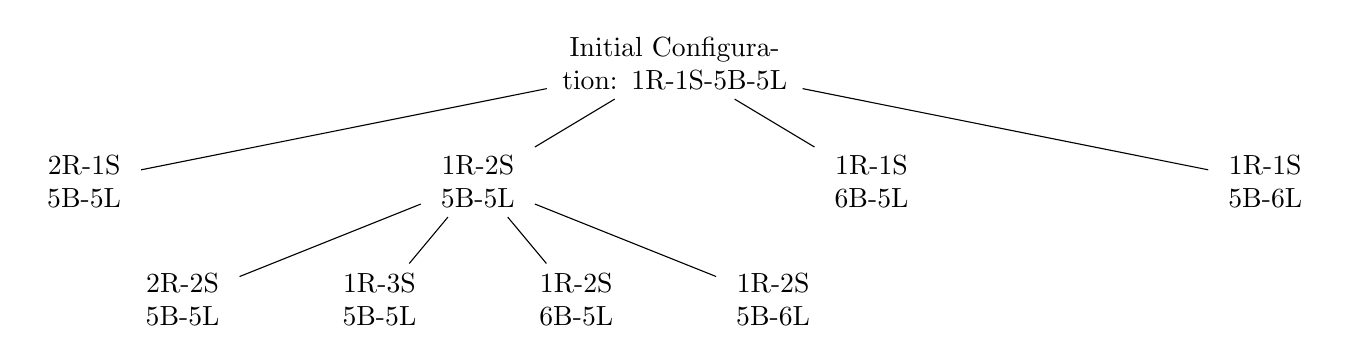
\begin{tikzpicture}[
      level distance=1.5cm,
      level 1/.style={sibling distance=5cm},
      level 2/.style={sibling distance=2.5cm}]
    \node[text width=3.0cm, align=center] {Initial Configuration:  1R-1S-5B-5L }
        child 
          { node [text width=1.2cm, align=center]{2R-1S 5B-5L} }
        child 
          { node [text width=1.2cm, align=center]{1R-2S 5B-5L} 
            child { node [text width=1.2cm, align=center]{2R-2S 5B-5L} }
            child { node [text width=1.2cm, align=center]{1R-3S 5B-5L} }
            child { node [text width=1.2cm, align=center]{1R-2S 6B-5L} }
            child { node [text width=1.2cm, align=center]{1R-2S 5B-6L} }
          }
        child 
          { node [text width=1.2cm, align=center]{1R-1S 6B-5L} }
        child 
          { node[text width=1.2cm, align=center] {1R-1S 5B-6L} };
  \end{tikzpicture}
  \caption{Example decision tree; configurations are represented as nodes. 
           Abbreviation of $R$,$S$,$B$, and $L$ represent ribs, spars, bulkheads, and
           longerons, respectively.}
  \label{fig_example_tree}
\end{figure}

This process is an extension of that used in 
\cite{clough_automated_wing_internal_structure_placement_guided_by_FEA}.
The python script \texttt{GRASP}\footnote{\texttt{GRASP} repository at \texttt{github.com/JustinClough/grasp}},
was again used to implement the design flow logic
and operate the branch-and-cut algorithm.
The design flow, shown in Figure \ref{fig_design_flow}
consisted of three main steps:
geometry creation, geometry management and discretization,
and FE analysis.

\begin{figure}[H]
  \centering
  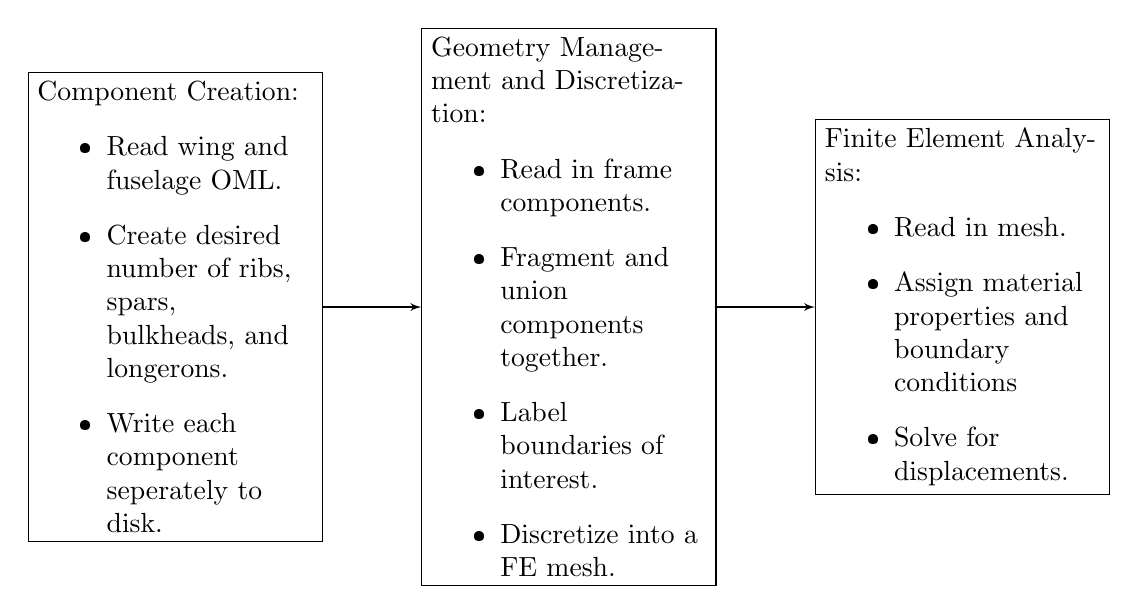
\begin{tikzpicture}[node distance = 5cm, auto]
    % Blocks
    \node [block] (geom) 
    {
      Component Creation:
      \begin{itemize}
        \item Read wing and fuselage OML.
        \item Create desired number of ribs, spars,
              bulkheads, and longerons.
        \item Write each component seperately to disk.
      \end{itemize}
    };
    \node [block, right of=geom] (mesh) 
    {
      Geometry Management and Discretization:
      \begin{itemize}
        \item Read in frame components.
        \item Fragment and union components together.
        \item Label boundaries of interest.
        \item Discretize into a FE mesh.
      \end{itemize}
    };
    \node [block, right of=mesh] (fea)  
    {
      Finite Element Analysis:
      \begin{itemize}
        \item Read in mesh.
        \item Assign material properties and boundary conditions
        \item Solve for displacements.
      \end{itemize}
    };
    % Lines
    \path [line] (geom) -- (mesh);
    \path [line] (mesh) -- (fea);
  \end{tikzpicture}
  \caption{Automatic design flow logic and steps. Adapted from 
          \cite{clough_automated_wing_internal_structure_placement_guided_by_FEA}. }
  \label{fig_design_flow}
\end{figure}

\noindent
Template input files were created for each of the subprograms used.
The python script edited each file for the desired problem configuration.
It then called each subprogram in the order to execute the design flow.

The first step of geometry creation was done by the script based geometry
kernel \texttt{Engineering Sketch Pad} (\texttt{ESP}) 
\cite{haimes_ESP_solid_modeling_feature_based_web_enabled_system_param_geom}.
The base geometry of the X-15 aeroplane, borrowed from 
\cite{gochenaur_rapid_geometry_generation_and_basic_comparison_x15},
and variations of it were used for this study.
Only the right half of the fuselage and right wing were
used to leverage the left-right symmetry of the vehicle.
Rib, spars, bulkheads, and longerons were created from the 
OML with specified thickenesses.
The frame components were then each writen to disk
and read into \texttt{Gmsh} 
\cite{geuzaine_GMSH_3D_FE_mesh_generator}.
This software joined all components together and
labeled all surfaces of interest.
These surfaces were later used to assign boundary 
condition in the FE analysis.
The geometry was then discretized into a FE mesh and written to disk.
This mesh was then read into \texttt{Albany} which
solved the FE problem
\cite{salinger_albany_using_component_based_design_to_dev_flex_multiphysics}.
The FE problem used a linear elastic material model to 
calculate the deformation of the structure.
Each of these step of the design flow are described 
in the following subsections.

\subsection{Parametric Geometry Creation}
The original functionality of \texttt{GRASP} was
used for rib and spar placement within the wing
\cite{clough_automated_wing_internal_structure_placement_guided_by_FEA}.
A wing root cap %TODO: citation needed?
was then added which attached to the roots of the spars.
Two sets of two functions were written in \texttt{ESP}
to allow the user to parametrically place bulkheads and 
longerons for any fuselage OML.
One function creates a single bulkhead at a percent length
from the nose of the fuselage;
another function evenly places a user defined number
of these bulkheads throughout the length of the fuselage.
A similar pair of functions were created for longeron 
placement. 
Here a percent rotation was defined for the 
center of each longeron and they were placed 
evenly throughout the circumference of the fuselage.

A template base input script was manually created and automatically 
edits for each problem configuration by the python script.
The \texttt{ESP} executable was then called as a subprocess.
The ribs, spars, bulkheads, and longerons were created by 
the scripts and written to disk as \texttt{.stp} files
\cite{iso_10303_21_2016_step_files}.
Each component was individually written as its own file.
The generic method was that file \texttt{$C$\_$N$.stp}
contained all geometric information of component type $C$ 
(rib, spar, bulkhead, or longeron) and number $N$.
In addition to the frame components,
a wing root cap was constructed to connect
the wing to the fuselage.
When finished, the output was checked for errors.

The original geometry of the X-15 (borrowed from 
\cite{gochenaur_rapid_geometry_generation_and_basic_comparison_x15})
and parametric variations of it were used.
The base geometry and the two variations considered
are shown in Figure \ref{fig_x15_external_base}
and \ref{fig_x15_external_variations}.

\begin{figure}[H] 
  \centering
    \includegraphics[width=0.95\textwidth, keepaspectratio]
    {x15_external_base}
  \caption{ Geometry of the base X-15 with the tail and cockpit removed.}
  \label{fig_x15_external_base}
\end{figure}

\begin{figure}[H] 
  \centering
  \subfigure[Doubled wing span.]
    {
      \includegraphics[width=0.95\textwidth, keepaspectratio]
      {x15_external_doubled_span}
    }
  \subfigure[Doubled fuselage diameter.]
    {
      \includegraphics[width=0.95\textwidth, keepaspectratio]
      {x15_external_doubled_fuselage_diameter}
    }
  \caption{
      Geometries of the two parametric variations of the X-15.
      One has a doubled wing span, the other with doubled fuselage diameters.}
  \label{fig_x15_external_variations}
\end{figure}

\noindent
One variation is a doubling the wing span 
(as measured from tip to fuselage, perpendicular to airflow)
and the other is a doubling of fuselage diameters.
The variations of the geometry are included to show two things.
First, the ability of the \texttt{GRASP} program to 
handle geometry that may be parametrically changed 
throughout the design process.
Second, that variations in the OML yield corresponding variations in 
structural layout.

\subsection{Geometry Management and Discretization}
A script template for \texttt{Gmsh} 
was manually created 
and automatically edited for each frame configuration.
The script first read the wing root cap \texttt{.stp} file from disk.
Next, it read the first spar from disk and used boolean 
fragmentation and unions to form a single volume
from the two components. 
This was repeated for the remainder of the spars.
Ribs were then added to the spar and wing cap
in a similar manner until the wing frame was completed.
Bulkheads and finally longerons were then added to the
frame using the same process.
The initial number of bulkheads was automatically chosen
such that at least one bulkhead would intersect 
and support the wing root cap.

Physical surfaces that would be assigned boundary conditions 
during the FE analysis were identified and labeled.
The wing underside was labeled first.
This was done by iterating through all surfaces after 
the wing frame was combined but before fuselage components 
were added.
The surface with lowest bounding box was labeled as the 
wing underside.
The mirror faces of the bulkheads were also each labeled.
This was done by searching for faces within a thin
bounding box near the expected bulkhead locations.

The combined and labeled geometry was then discretized 
into second order tetrahedral finite elements.
The mesh size was dictated such that two of these
second order element spanned any geometric feature.
The meshing was done in parallel using the
inbuilt multi-thread feature of \texttt{Gmsh}.


\subsection{Finite Element Analysis}
The program \texttt{Albany} was given two input files for 
each configuration. 
Templates were manually created for each file and edited 
automatically through the python script.
One file listed boundary conditions and linear solver
parameters.
The other file listed material properties and material 
model type.

The wing underside was assigned a
Neumann boundary condition of a defined pressure distribution
to match expected in flight conditions.
An additional body load was exerted throughout the
structure to represent the weight of the components.
Homogeneous Dirichlet boundary conditions were 
prescribed on the bulkhead faces such that
they remained flush with the plane of symmetry.
% TODO: double check this BC
All degrees of freedom on the center most
bulkhead face were also assigned a
homogeneous Dirichlet boundary condition.
This served to eliminate any rigid body motion in the model.

The material model used was linear elastic.
The user was able to define both the
Young's modulus and Poisson ratio for the material.
The same material model and properties were used throughout
the frame.
Ten node composite tetrahedral elements were used
\cite{ostien_10_node_comp_tet_FE_for_solid_mechanics}.
Testing has shown that these element definitions do not 
show shear locking effects typical of other 
formulations for similar finite elements 
when modeling thin structures.
Once the input files were prepared,
\texttt{Albany} was called as parallel 
subprocess using the Message Passing Interface (\cite{ mpi_standard_1994})
from the main python script.


\section{Preliminary And Planned Results} \label{sec_results}
A frame layout for the base X-15 is shown in 
Figure \ref{fig_prelim_frame}.
This frame was created automatically using the 
parametric geometry kernel \texttt{ESP}
and the functions written to 
create the ribs, spars, bulkheads and longerons
with even spacing.

\begin{figure}[H] 
  \centering
    \includegraphics[width=0.95\textwidth, keepaspectratio]
    {x15_prelim_frame}
  \caption{ Preliminary frame layout for the X-15.}
  \label{fig_prelim_frame}
\end{figure}

\noindent
This configuration of 5 ribs, 4 spars, 10 bulkheads, and 10 longerons
shows that the work flow can create the geometry as needed.
Note that not all 10 longerons are shown as
only have of the vehicle is modeled.
Also, work has been completed which allows both the \texttt{Gmsh}
and \texttt{Albany} subprocesses to each be called 
with multi-thread and parallel capabilities, respectively.
Additional work includes the following items:
\begin{itemize}
  \item Use boolean fragmentations and unions to form a solid
        geometry, then discretize using the \texttt{Gmsh} scripting 
        language.
  \item Find and label boundaries of interest for use with boundary 
        conditions during the FE analysis with the \texttt{Gmsh} 
        scripting language.
  \item Assign boundary conditions and body loads of interest in 
        the \texttt{Albany} input files.
  \item Conduct a test case for each of the three geometries 
        (the base and two variations) considered.
\end{itemize}

\noindent
For each of the geometries considered, 
the solution time, timing breakdown,
wing tip deflection, and number of finite elements
at each configuration will be plotted.
Similarities and difference between and within 
the solution configurations will be denoted.

% \section{Discussion and Closing Remarks} \label{sec_closing_remarks}
% discussion text

% \section{Future Work} \label{sec_future}
% future work text
% 
% \section*{Acknowledgments}
% The authors thank the DoD Science, Mathematics, And 
% Research for Transformation (SMART) Scholarship
% for Service Program which sponsored this work.


\bibliography{monolith.bib}

\end{document}
